
\section{Organisation}

\begin{frame}
  {Literatur | Einführungen}
  \onslide<+->
  \begin{itemize}[<+->]
    \item \alert{\citet{ChierchiaMcconnellginet2000}} | GB-orientiert, nur die Kapitel von Chierchia
    \item \alert{\citet{ParteeEa1990}} | wichtige Grundlagen (Algebra, Logik), viele Druckfehler
  \end{itemize}
\end{frame}

\begin{frame}
  {Literatur | weitere Empfehlungen}
  \onslide<+->
  \begin{itemize}[<+->]
    \item \alert{\citet{Bucher1998}} | lesbare Logik-Einführung auf Deutsch
    \item \alert{\citet{DowtyEa1981}} | tolle Montague-Einführung von seinen Schülern
    \item \alert{\citet{Carpenter1997}} | prima Hardcore-Einführung mit Kategorialgrammatik
    \item \alert{\citet{Gutzmann2019}} | aktuelle Einführung auf Deutsch
  \end{itemize}
\end{frame}


\begin{frame}
  {Seminarverlauf}
  \onslide<+->
  \begin{enumerate}[<+->]\Lf\scriptsize
    \item \alert{9.10.2023} Diskussion: Wie schlussfolgern wir? Wie hängen unser Schlussfolgerungen mit Semantik zusammen?
    \item \alert{26.10.2023} Referentielle Semantik (Folien 2)
    \item \alert{02.11.2023} Mengen- und Funktionstheorie (Folien 3)
    \item \alert{09.11.2023} Aussagenlogik (Folien 4)
    \item[\rule{1.2em}{1.2em}] \raisebox{2pt}{\grau{16.11.2023 Ausfall wegen Dienstreise}}
    \item \alert{23.11.2023} Prädikatenlogik (Folien 5)
    \item \alert{30.11.2023} Quantifikation und modelltheoretische Semantik (Folien 6)
    \item \alert{07.12.2023} Einfach getypte höherstufige λ-Sprachen (Folien 7)
    \item \alert{14.12.2023} Intensionalität (Folien 8)
    \item \alert{21.12.2023} Tempus und Modalität (Folien 9)
    \item[\rule{1.2em}{1.2em}] \raisebox{2pt}{\grau{28.12.2023 Weihnachtsferien}}
    \item[\rule{1.2em}{1.2em}] \raisebox{2pt}{\grau{04.01.2024 Weihnachtsferien}}
    \item \alert{11.01.2024} Montagues intensionale Logik (Folien 10)
    \item \alert{18.01.2024} \gruen{\textit{The Proper Treatment of Quantification in Ordinary English} (Montague 1973)}
    \item \alert{25.01.2024} \gruen{\textit{Generalized Quantifiers and Natural Language} (Barwise \& Cooper 1981)}
    \item \alert{01.02.2024} \gruen{\textit{The Algebra of Events} (Bach 1986)}
    \item[\rule{1.2em}{1.2em}] \raisebox{2pt}{\grau{08.02.2024 Klausurenwoche\slash Einzelbesprechungen}}
  \end{enumerate}
\end{frame}

\begin{frame}
  {Prüfungen}
  \onslide<+->
  \onslide<+->
  Einheitlicher Inhalt für alle Modul- und Examensprüfungen:\\
  \Zeile
  \begin{enumerate}[<+->]
    \item eine oder zwei inhaltlichen Fragen zu den Themen der \textit{Sprachphilosophie}\\
      \grau{\footnotesize Die Liste der relevanten Texte wird rechtzeitig vor den Prüfungen eingeschränkt.}
    \item eine Logik-Aufgabe (natürliche Deduktion) -- \alert{außer in mündlichen Prüfungen}
    \item eine Semantik-Aufgabe (kompositionale Modellierung eines Satzes)
  \end{enumerate}
  \Zeile
  \onslide<+->
  \grau{Hausarbeiten nach Absprache.}
\end{frame}

\section{Schlussfolgern}

\begin{frame}
  {Was folgt aus A?}
\end{frame}

\begin{frame}
  {Folgt B aus A? | Einfache Fälle}
\end{frame}

\begin{frame}
  {Folgt B aus A? | Schwierigere Fälle}
\end{frame}

\begin{frame}
  {Folgt B aus A? | Grammatik}
\end{frame}

\begin{frame}
  {Woher wissen Sie das?}
\end{frame}

\begin{frame}
  {Weltwissen vs.\ Logik}
\end{frame}

\begin{frame}
  {Inferenz | Abduktion}
\end{frame}

\begin{frame}
  {Inferenz | Induktion}
\end{frame}

\begin{frame}
  {Inferenz | Deduktion}
\end{frame}

\begin{frame}
  {Deduktion, Logik und Modelltheorie}
\end{frame}

\section{Grundfragen}

\begin{frame}
  {Begriffe von "`Bedeutung"'}
  \onslide<+->
  \onslide<+->
  Die Bedeutung eines Ausdrucks ist \ldots\\
  \Zeile
  \begin{itemize}[<+->]
    \item \ldots\ die Idee, die er vermittelt
    \item \ldots\ die mentale Repräsentation, die er erzeugt
    \item \ldots\ was mit ihm bewirkt werden soll
    \item \ldots\ \gruen<7->{die Menge der Dinge, auf die er verweist}
  \end{itemize}
\end{frame}

\begin{frame}
  {Mögliche "`Semantiken"'}
  \onslide<+->
  \onslide<+->
  Semantik untersucht \ldots\\
  \begin{itemize}[<+->]
    \item \ldots\ intellektuelle Konzepte, die überwiegend introspektiv erforschbar sind
    \item \ldots\ die kognitive Verarbeitung und Repräsentation von Bedeutung
    \item \ldots\ die Funktion von Ausdrücken in Kommunikationssituationen
    \item \ldots\ \gruen<7->{Beziehungen zwischen Ausdrücken und Objekten und\\
      die Art der Kombination von Ausdrücken zur komplexeren Ausdrücken}
  \end{itemize}
\end{frame}

\begin{frame}
  {Konkrete Fragen in diesem Seminar}
  \onslide<+->
  \onslide<+->
  Es dreht sich alles um die Beziehung von Sprache zur Welt!\\
  \Zeile
  \begin{itemize}[<+->]
    \item Auf welche Klassen von Objekten \alert{referieren} auf welche Klassen von Ausdrücken?
    \item Wann sind Sätze wahr? (auch als Phänomen der \alert{Referenz}!)
    \item Wie verhält sich die logische Struktur von Sätzen zu ihrem Informationsgehalt?
    \item Wie können Sätze eindeutig interpretiert werden,\\
      auch wenn sie mehrere Lesarten haben?
  \end{itemize}
\end{frame}

\begin{frame}
  {\rot{Keine} Fragen in diesem Seminar}
  \onslide<+->
  \begin{itemize}[<+->]
    \item Was ist die "`Bedeutung"' von Wörtern und Sätzen jenseits ihrer Referenz?
    \item Wie verarbeitet das Gehirn Bedeutungen?
    \item Wie sind Diskurse strukturiert?
  \end{itemize}
\end{frame}

\section{Programmatisches Schlussbild}

\begin{frame}
  {Programmatisches Schlussbild | Frage}
  \onslide<+->
  \onslide<+->
  \centering\large
  Sind Sie nun kognitiver Linguist,\\
  der sich für (probabilistische) \alert{mentale Kategorien} interessiert,\\
  \Halbzeile
  \onslide<+->
  oder glauben Sie daran,\\
  dass Sprache \alert{unabhängig vom Menschen logische Eigenschaften} hat?\\
  \onslide<+->
  \Zeile
  \orongsch{Beides gleichzeitig geht ja nun wirklich nicht!}
\end{frame}

\begin{frame}
  {Programmatisches Schlussbild | Exkurs I}
  \onslide<+->
  \onslide<+->
  \alert{Kognition}\\
  \Viertelzeile
  \begin{itemize}[<+->]
    \item basierend auf Ähnlichkeiten von wahrgenommenen Objekten
    \item optimiert für schnelle Mustererkennung \alert{in allen Bereichen}
    \item unscharfe Klassenbildung und Segmentierung der Ontologie
    \item parallele Verarbeitung (meistens mehrere Areale beteiligt)
  \end{itemize}
  \Halbzeile 
  \onslide<+->
  \alert{Symbolische Systeme}\\
  \Viertelzeile
  \begin{itemize}[<+->]
    \item diskrete Symbole, wohldefinierte Semantik
    \item scharf getrennte Klassen von Symbolen
    \item eindeutige Referenz auf ontologische Objekte
    \item intrinsische (nicht emergente) logische Eigenschaften\\
      \grau{(Axiomatik, Schlussregeln usw.)}
    \item sequentielle Verarbeitung\slash statische Deklaration\\
      \grau{(\zB Python oder PROLOG; parallele Verarbeitung immer linearisierbar)}
  \end{itemize}
\end{frame}

\begin{frame}
  {Programmatisches Schlussbild | Exkurs II}
  \onslide<+->
  \onslide<+->
  Klassisches kognitives Modell: \alert{Prototypentheorie} \grau{\citep{Rosch1973}}\\
  \onslide<+->
  \Zeile
  \alert{Diskretes Symbol}: \gruen{Vogel} \onslide<+-> \ldots\ und demgegenüber \ldots\\
  \onslide<+->
  \alert{Graduelles kognitives Konzept} basierend auf Ähnlichkeiten\slash Prototypen:\\
  \onslide<+->
  \Halbzeile
  \begin{minipage}{0.9\textwidth}
  \centering
    $\vcenter{\hbox{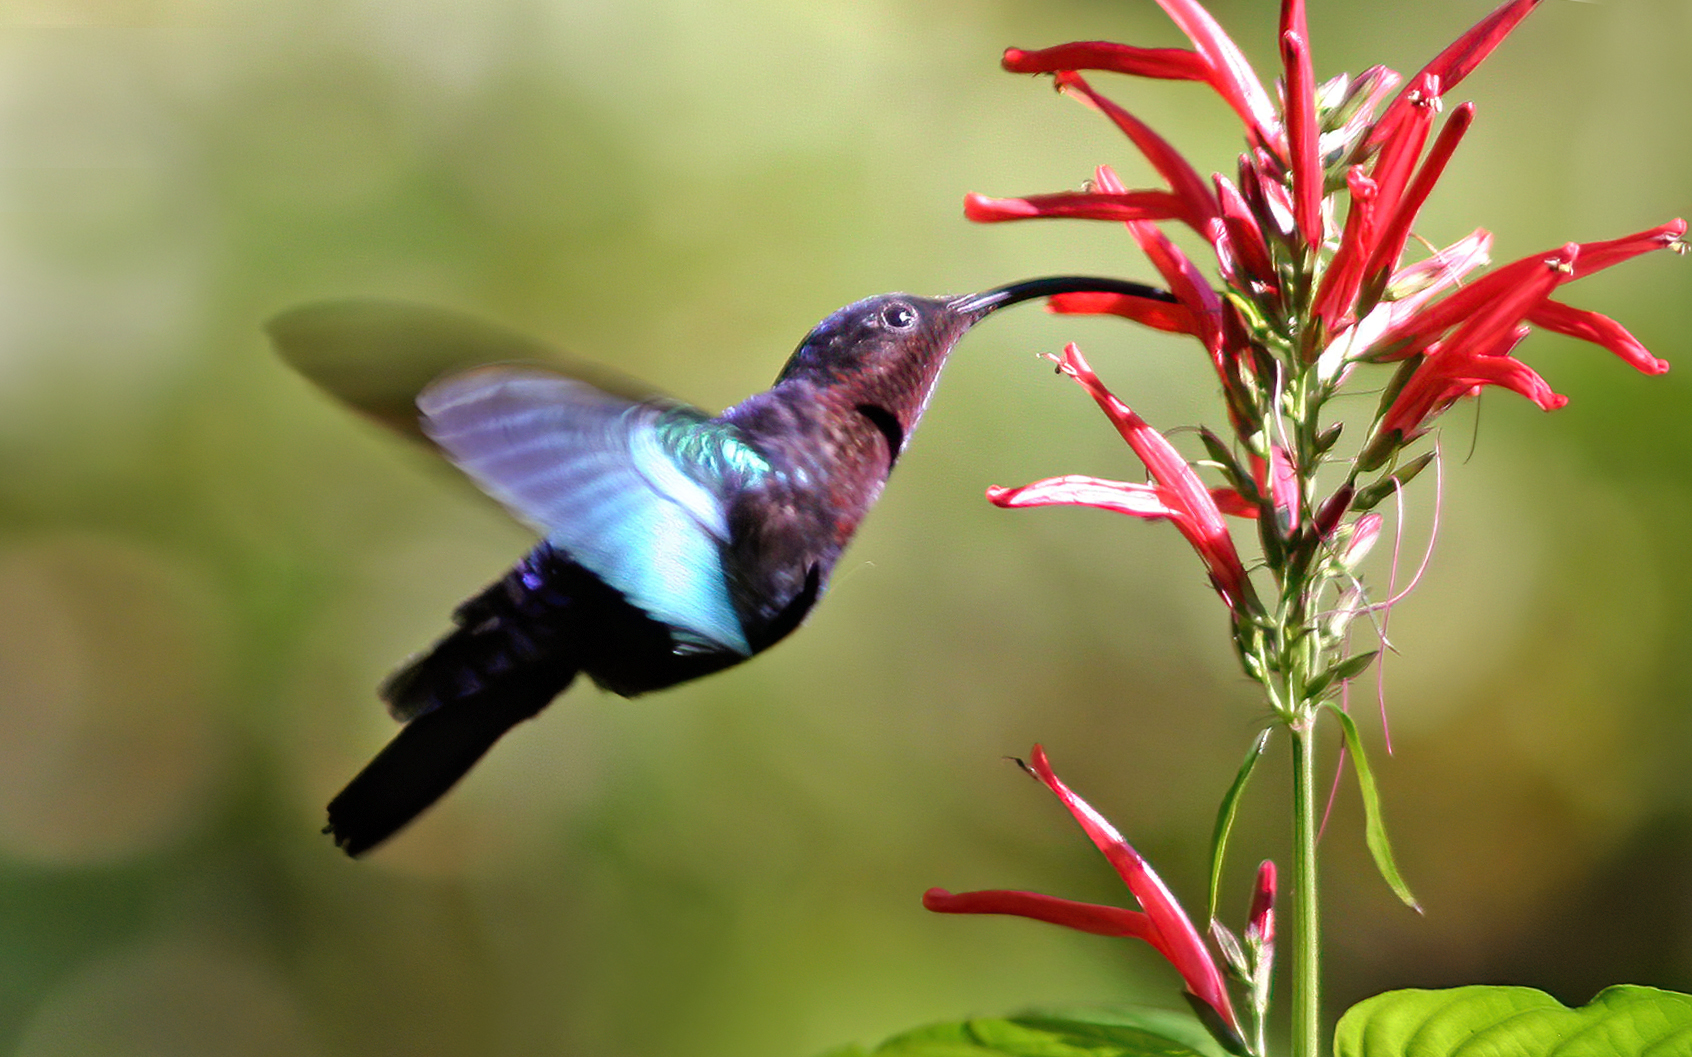
\includegraphics[width=0.2\textwidth]{\GRAPHPATH/kolibri}}}$
    \onslide<+->
    \hspace*{0.025\textwidth}>\hspace*{0.025\textwidth}
    $\vcenter{\hbox{\includegraphics[width=0.1\textwidth]{\GRAPHPATH/kiwi}}}$
  \end{minipage}
\end{frame}

\begin{frame}
  {Programmatisches Schlussbild | Antwort}
  \onslide<+->
  \onslide<+->
  Die ewige Schwachsinnsfrage: Sind Kiwis und Pinguine nun \gruen{Vögel} oder nicht?\\
  \Viertelzeile
  \grau{Nur getoppt von: Erdbeeren sind gar keine Beeren, sondern Sammelnussfrüchte.}\\
  \Zeile
  \begin{itemize}[<+->]
    \item \alert{Kognition} | \orongsch{intrinsisch nicht diskret}, sondern ähnlichkeitsbasiert und \orongsch{parallel}
      \begin{itemize}[<+->]
        \item \orongsch{Netzwerkarchitektur}
      \end{itemize}
      \Halbzeile
    \item \alert{Symbole} = Phone, Morphe, Wörter, Phrasen, \ldots | \orongsch{intrinsisch} diskret und \orongsch{linear}
      \begin{itemize}[<+->]
        \item \orongsch{akustisches} Medium | Sagen Sie mal zwei Wörter gleichzeitig!
        \item \orongsch{schriftliches} Medium | Lesen Sie mal \textit{Zettels Traum}!
      \end{itemize}
    \Halbzeile
    \item[\ding{222}] Da wir nur akustisch oder über schriftliche Artefakte kommunizieren können,\\
      \alert{muss das Sprachsystem symbolisch sein}.
    \item[\ding{222}] Da es architekturbedingt nur nicht-symbolisch verarbeiten kann,\\
      \alert{muss das Gehirn symbolische Systeme so gut wie nötig und möglich emulieren}.
  \end{itemize}
\end{frame}


\begin{frame}
  {Programmatisches Schlussbild | Ausführung}
  \onslide<+->
  \onslide<+->
  Auch nicht-verschriftete Sprache muss medial bedingt logische Eigenschaften haben.\\
  \onslide<+->
  Kulturell bilden sich stärker symbolische Modi aus, vor allem durch Schrift.\\
  \grau{\footnotesize Norm, Selbst- und Fremdkorrektur, Textplanung, intensionale Definitionen, Explizierung, \ldots}\\
  \grau{\footnotesize Warum wird das vor allem im Kontext von Schule, Fremdsprache und Bildungssprache diskutiert?}\\
  \onslide<+->
  \Zeile
  \Halbzeile
  \centering 
  \begin{tabular}[h]{cc}
    \grau{(= spontane Sprachproduktion)} & \\
    \orongsch{weniger symbolische Eigenschaften} & \small \orongsch{informelle Alltagssprache} \\
    \onslide<+->
    \textcolor{orgrA}{\faArrowDown} &\large \textcolor{orgrA}{formelle Alltagssprache} \\
    \onslide<+->
    \textcolor{orgrB}{\faArrowDown} &\Large \textcolor{orgrB}{Bildungssprache} \\
    \onslide<+->
    \textcolor{orgrC}{\faArrowDown} &\LARGE \textcolor{orgrC}{Wissenschaftssprache} \\
    \onslide<+->
    \textcolor{orgrD}{\faArrowDown} &\huge \textcolor{orgrD}{Orthosprache} \\
    \onslide<+->
    \gruen{mehr symbolische Eigenschaften} & \gruen{\Huge formales System} \\
    \grau{(= reflektierte Sprachproduktion)}  & \\
  \end{tabular}
\end{frame}

\begin{frame}
  {Und was ist denn nun mit Kiwis und Pinguinen?}
  \onslide<+->
  \onslide<+->
  Unser Verständnis der Welt führt zu genaueren und diskreten Kategorisierungen,\\
  wo dies nötig ist. \alert{Die Sprache folgt diesem Maß an Genauigkeit und Diskretheit!}\\
  \Zeile
  \onslide<+->
  \centering
  \begin{minipage}{0.9\textwidth}
  \centering
    $\vcenter{\hbox{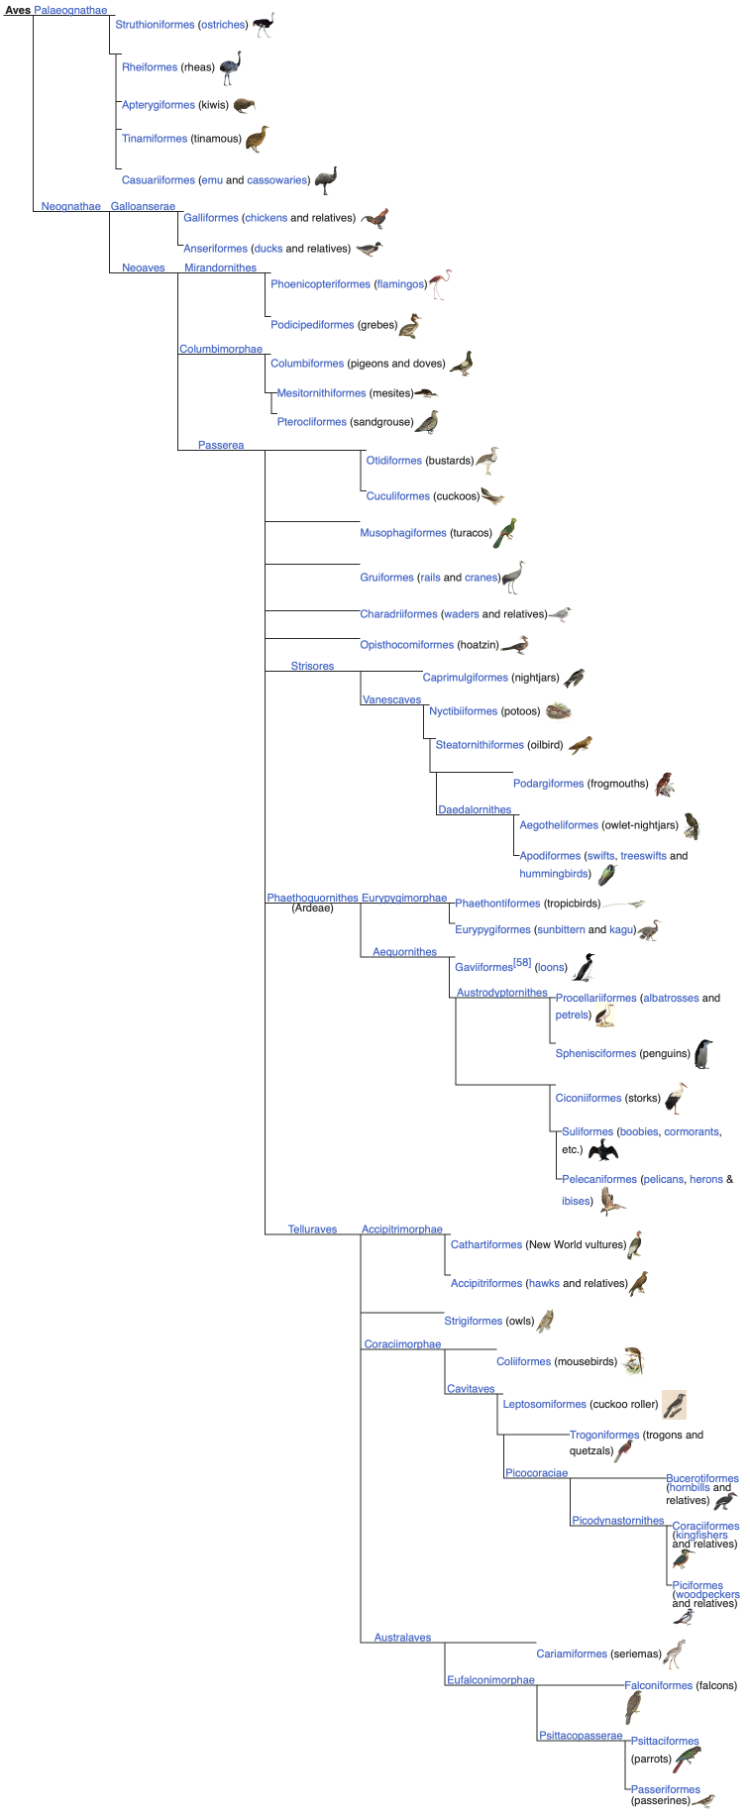
\includegraphics[height=0.7\textheight]{\GRAPHPATH/birds50}}}$\hspace{0.1\textwidth}
      \only<3>{$\vcenter{\hbox{\rule{0.4\textwidth}{0em}}}$}%
      \only<4>{$\vcenter{\hbox{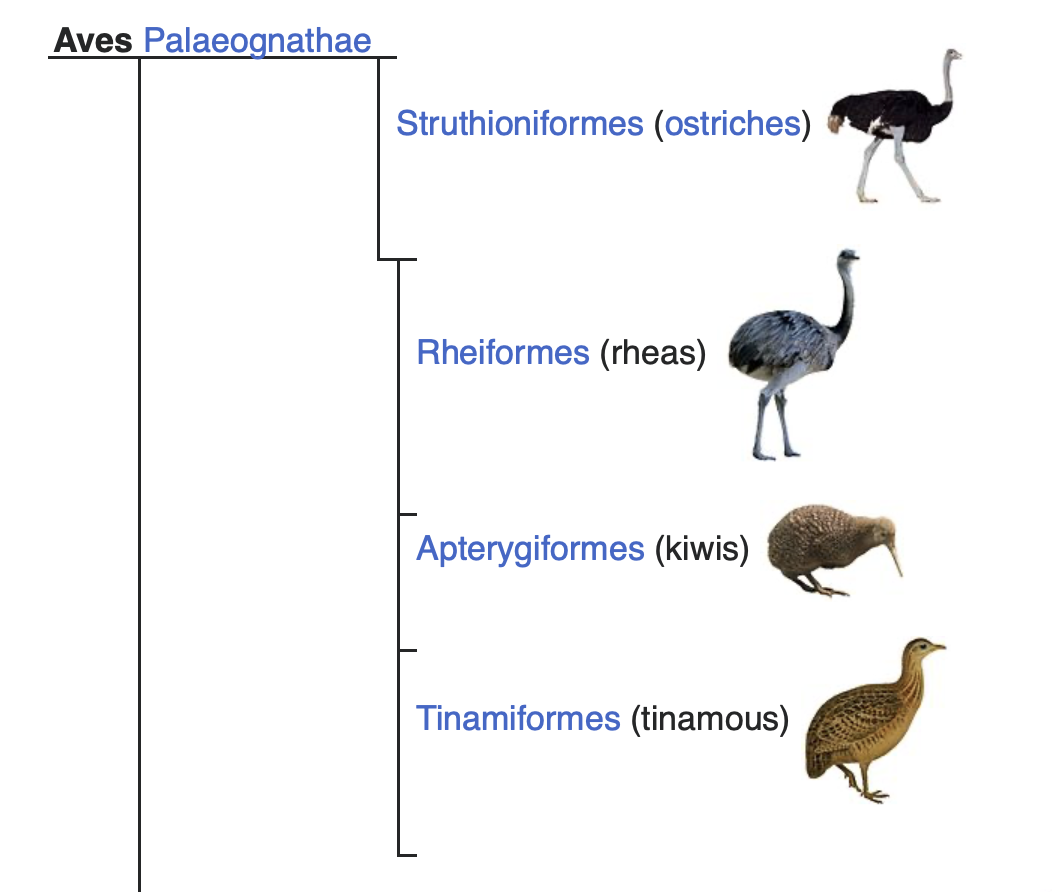
\includegraphics[width=0.4\textwidth]{\GRAPHPATH/kiwis}}}$}%
      \only<5>{$\vcenter{\hbox{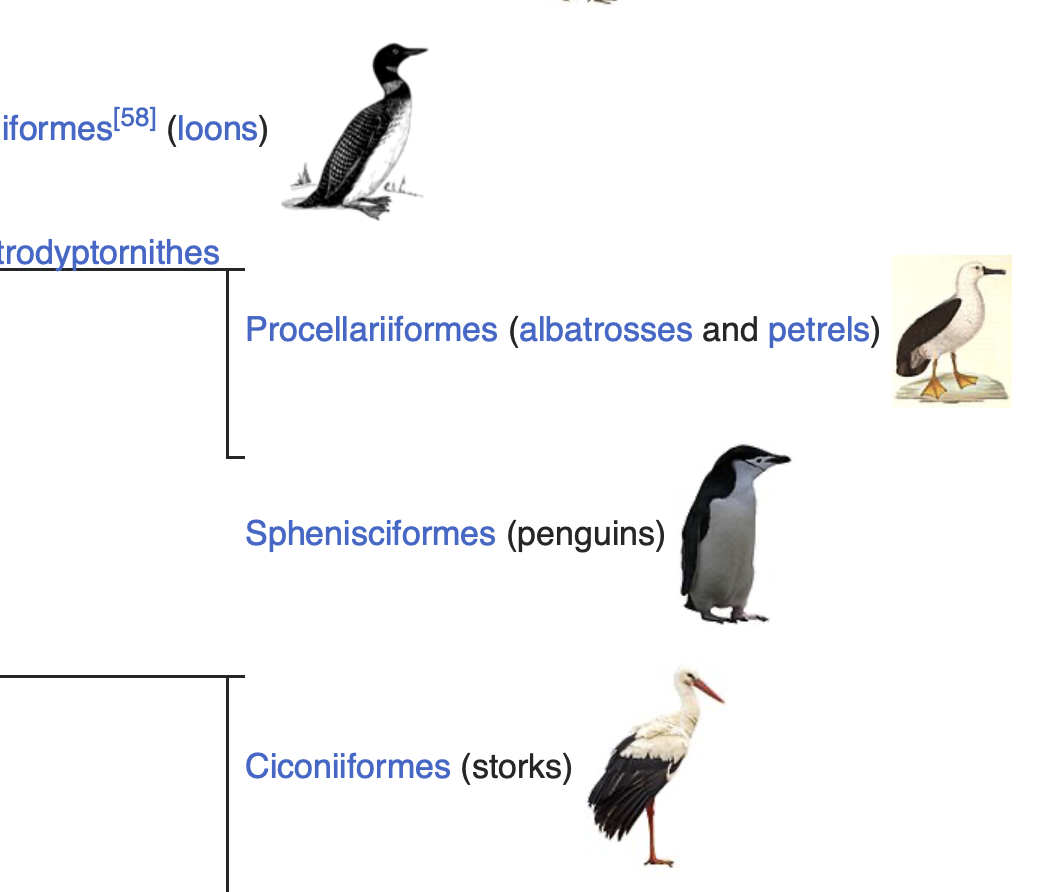
\includegraphics[width=0.4\textwidth]{\GRAPHPATH/penguins}}}$}
  \end{minipage}
\end{frame}

\begin{frame}
  {Letzte Folie}
  \onslide<+->
  \begin{itemize}[<+->]
    \item Viele Missverständnisse in der Linguistik basieren darauf,\\
      dass das eben Gesagte nicht dem allgemeinen Forschungsprogramm zugrundeliegt.
    \item Die Doppelnatur von Sprache führt dazu, dass sowohl rein formale Linguistik\\
      und sogenannte kognitive Linguistik scheinbar erfolgreich sind.
    \item Im Prinzip läuft aber die Linguistik aktuell weitgehend ins Leere.
      \Halbzeile
    \item \alert{Modelltheoretische Semantik beschreibt einen essentiellen Teil von Sprache!}
    \item \alert{Sie modelliert logische Eigenschaften und den Bezug zur realen objektiven Welt.}
      \Halbzeile
    \item \grau{Ganz am Rande zu generativer AI \ldots}
      \begin{itemize}[<+->]
        \item \grau{Erfolg | Sie modelliert völlig natürliche Grammatik.}
        \item \grau{\ldots\ also alle Grammatiker bitte setzen!}
        \item \grau{Misserfolg | Sie weiß nichts über die Welt,\\
          es wirkt nur so wegen des immensen sprachlichen Inputs.}
        \item \grau{\ldots\ eine Art fancy Papagei.}
      \end{itemize}
  \end{itemize}
\end{frame}
